\documentclass[12pt,titlepage]{article}
\usepackage[margin=1in]{geometry}
\usepackage[utf8]{inputenc}
\usepackage{amsmath}
\usepackage{graphicx}
\usepackage{hyperref}
\usepackage{titlesec}
\usepackage{booktabs}

\titleformat{\section}{\normalfont\Large\bfseries}{\thesection}{1em}{}
\titleformat{\subsection}{\normalfont\large\bfseries}{\thesubsection}{1em}{}

\begin{document}

% --- HALAMAN JUDUL ---
\begin{titlepage}
    \centering
    \vspace*{2cm}
    {\LARGE\bfseries PROPOSAL PRE-FINAL PROJECT}\\[0.5cm]
    {\Large\bfseries PENGEMBANGAN APLIKASI ANDROID}\\[1.5cm]
    
    {\Large\scshape ID APLIKASI: LibrePulse}\\[0.3cm]
    {\large Port-Level Loop Isolation Interface for LibreNMS}\\[3cm]
    
    
\includegraphics[width=5cm]{Unida.png}\\[1.5cm]
    \vspace{1cm}
    \begin{tabular}{ll}
        \textbf{Nama} & : Muhammad Dafi Al Haq \\
        \textbf{NIM}  & : 452024611067 \\
        \textbf{Kelas} & : A2 \\
        \textbf{Dosen} & : Wahid Alfaridsi Achmad Zein M.Kom. \\
    \end{tabular}
    
    \vfill
    {\large PROGRAM STUDI TEKNIK INFORMATIKA}\\[0.2cm]
    {\large UNIVERSITAS DARUSSALAM GONTOR}\\[0.2cm]
    {\large 19 Juli 2026}
\end{titlepage}

% --- KONTEN PROPOSAL ---

\section{Judul \& Latar Belakang}

\subsection{Nama Aplikasi}
Aplikasi ini diberi nama \textbf{LibrePulse}, sebuah platform \textit{mobile network utility client} berbasis Android yang terintegrasi dengan REST API LibreNMS untuk penanganan insiden \textit{switching loop} pada tingkat port fisik.

\subsection{Masalah yang Ingin Diselesaikan}
Ketika terjadi gangguan jaringan akibat \textit{looping} (\textit{broadcast storm}), protokol \textit{Spanning Tree Protocol} (STP) atau \textit{loop protection} pada \textit{Managed Switch} dan \textit{RouterBoard} (RB) akan otomatis mengisolasi dengan mematikan (\textit{blocking/disable}) **satu port spesifik** yang menjadi sumber masalah. Dalam kondisi ini, perangkat utama secara makro tetap berstatus aktif (\textit{Up}), namun performa jaringan sektoral terganggu.

Proses \textit{troubleshooting} di lapangan saat ini memiliki kelemahan:
\begin{enumerate}
    \item \textbf{Ketiadaan Detail Port Makro:} Aplikasi monitoring standar hanya memberikan status global perangkat (\textit{Device Up/Down}). Teknisi tidak bisa mengetahui port spesifik mana yang mati terisolasi tanpa membuka laptop dan masuk ke CLI atau WinBox.
    \item \textbf{Penanganan Kasus Perangkat Mati Total:} Ketika perangkat utama mati (\textit{Device Down}), sistem monitoring sering kali membuang waktu dengan tetap mencoba melakukan \textit{polling} data port yang sebenarnya sudah tidak dapat diakses.
    \item \textbf{Masalah Sinyal Ruang Server:} Tidak adanya mekanisme penyimpanan data lokal (\textit{offline caching}) saat teknisi melakukan inspeksi fisik di ruang server bawah tanah yang kedap sinyal seluler.
\end{enumerate}

\subsection{Target Pengguna}
Target pengguna utama dari aplikasi ini adalah \textit{Network Engineers, System Administrators, Network Operations Center (NOC) Operators}, dan teknisi IT Support lapangan.

---

\section{Fitur Utama (Features List)}

Aplikasi LibrePulse mengimplementasikan lima fitur utama berikut:

\begin{itemize}
    \item \textbf{Global Network Health Summary (Header Dashboard):} Menampilkan penghitung biner status perangkat utama yang aktif dan mati (\textit{Device Up} dan \textit{Device Down}) secara *real-time* di bagian atas halaman utama.
    \item \textbf{Managed Device Dynamic List:} Menampilkan daftar seluruh Switch dan RouterBoard. Setiap kartu perangkat dilengkapi indikator biner jumlah port internal yang aktif dan mati (contoh: \textit{Up: 23 | Down: 1}).
    \item \textbf{Dead-Host Safety Handler:} Logika proteksi visual di mana jika perangkat utama berstatus mati (\textit{Down}), aplikasi otomatis mengunci indikator port menjadi kosong (\textit{Up: - | Down: -}) untuk menandakan data tidak dapat diakses.
    \item \textbf{Master-Detail Navigation Flow:} Mekanisme perpindahan halaman dari daftar perangkat menuju direktori port spesifik saat kartu perangkat diklik menggunakan parameter ID unik.
    \item \textbf{Port-Level Interface Directory:} Menampilkan daftar seluruh port fisik (contoh: \textit{Port 1} hingga \textit{Port 5}) lengkap dengan pemetaan IP Address dan indikator warna biner status (\textit{Green} = Normal, \textit{Red} = Down/Blocked).
    \item \textbf{Offline Room Database Cache:} Menyimpan snapshot status perangkat dan port terakhir secara lokal untuk menjamin operasional aplikasi tetap berjalan di area tanpa sinyal.
\end{itemize}

---

\section{Arsitektur \& Komponen Android}

Arsitektur aplikasi dibangun di atas pola \textbf{MVVM (Model-View-ViewModel)} dengan \textbf{Repository Pattern} untuk memastikan pemisahan logika kode yang bersih (\textit{Modern Android Development}):

\begin{table}[h]
    \centering
    \caption{Komponen Teknis Implementasi Aplikasi}
    \vspace{0.2cm}
    \begin{tabular}{lp{10cm}}
        \toprule
        \textbf{Komponen Android} & \textbf{Deskripsi Fungsi Teknis} \\
        \midrule
        \texttt{Activity / Fragment} & Mengelola dua layar utama: \textit{Dashboard Fragment} (Daftar Switch/RB) dan \textit{PortDetail Fragment} (Daftar Antarmuka \& IP Port). \\
        \texttt{Intent \& Navigation} & Mengalirkan data \textit{Device ID} secara aman antar-fragment menggunakan \textit{SafeArgs}. \\
        \texttt{Advanced RecyclerView} & Menampilkan daftar port secara dinamis menggunakan pembaruan \textit{DiffUtil} berdasarkan perubahan status biner (\textit{Up/Down}). \\
        \texttt{Retrofit \& Moshi} & Melakukan request asinkron ke \textit{endpoint} REST API LibreNMS (\texttt{/api/v0/devices}) untuk menarik data JSON perangkat dan port. \\
        \texttt{Room Database} & Mengelola persistensi data lokal (\textit{offline cache data}) untuk tabel \texttt{DeviceEntity} dan \texttt{PortEntity}. \\
        \texttt{Kotlin Coroutines} & Menangani proses *asynchronous threading* agar aktivitas *fetch data* dari API tidak memicu *UI freezing* pada *Main Thread*. \\
        \bottomrule
    \end{tabular}
\end{table}

---

\section{Rancangan Antarmuka (Wireframe/Mockup)}

Berikut adalah rancangan antarmuka \textit{low-fidelity} dari aplikasi \textbf{LibrePulse} yang mencakup halaman utama Dashboard dan Halaman Detail Port Perangkat:

\begin{figure}[htbp]
    \centering
    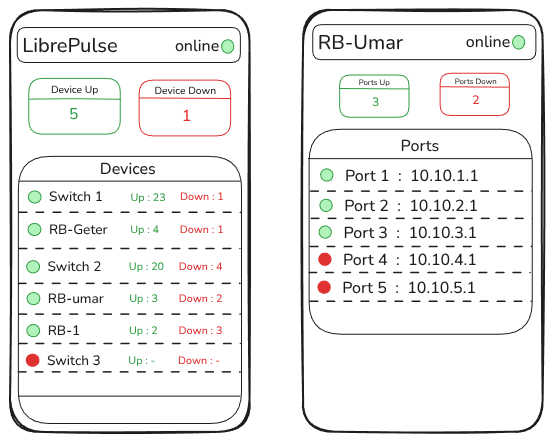
\includegraphics[width=0.9\textwidth]{mockup.png}
    \caption{Rancangan Antarmuka Utama (Dashboard) dan Halaman Detail Port LibrePulse}
    \label{fig:mockup_dashboard}
\end{figure}

Penjelasan fungsional komponen antarmuka pada Gambar~\ref{fig:mockup_dashboard}:
\begin{itemize}
    \item \textbf{Layar 1 (Dashboard Utama)}: Menampilkan ringkasan jumlah perangkat aktif/mati di bagian atas (\textit{Device Up: 5 | Device Down: 1}). Pada bagian list perangkat, item \texttt{Switch 3} mendemonstrasikan fitur \textit{Dead-Host Handler} di mana indikator port otomatis berubah menjadi kosong (\textit{Up: - | Down: -}) karena status utama perangkat berada dalam kondisi \textit{Down} (Merah).
    \item \textbf{Layar 2 (Detail Port Perangkat)}: Menampilkan halaman setelah kartu \texttt{RB-Umar} diklik. Bagian atas menyajikan total agregasi port internal (\textit{Ports Up: 3 | Ports Down: 2}), diikuti dengan daftar \textit{interface} fisik dari Port 1 sampai Port 5 lengkap dengan alokasi alamat IP masing-masing serta indikator warna status biner yang sinkron dengan halaman utama.
\end{itemize}

\end{document}
